% Options for packages loaded elsewhere
\PassOptionsToPackage{unicode}{hyperref}
\PassOptionsToPackage{hyphens}{url}
\PassOptionsToPackage{dvipsnames,svgnames,x11names}{xcolor}
\PassOptionsToPackage{space}{xeCJK}
\documentclass[
  11pt,
  a4paper,
]{article}
\usepackage{xcolor}
\usepackage[margin=20mm]{geometry}
\usepackage{amsmath,amssymb}
\setcounter{secnumdepth}{-\maxdimen} % remove section numbering
\usepackage{iftex}
\ifPDFTeX
  \usepackage[T1]{fontenc}
  \usepackage[utf8]{inputenc}
  \usepackage{textcomp} % provide euro and other symbols
\else % if luatex or xetex
  \usepackage{unicode-math} % this also loads fontspec
  \defaultfontfeatures{Scale=MatchLowercase}
  \defaultfontfeatures[\rmfamily]{Ligatures=TeX,Scale=1}
\fi
\usepackage{lmodern}
\ifPDFTeX\else
  % xetex/luatex font selection
  \setmainfont[]{DejaVu Serif}
  \setsansfont[]{DejaVu Sans}
  \setmonofont[]{DejaVu Sans Mono}
  \ifXeTeX
    \usepackage{xeCJK}
    \setCJKmainfont[AutoFakeBold=1.4]{Droid Sans Fallback}
  \fi
  \ifLuaTeX
    \usepackage[]{luatexja-fontspec}
    \setmainjfont[AutoFakeBold=1.4]{Droid Sans Fallback}
  \fi
\fi
% Use upquote if available, for straight quotes in verbatim environments
\IfFileExists{upquote.sty}{\usepackage{upquote}}{}
\IfFileExists{microtype.sty}{% use microtype if available
  \usepackage[]{microtype}
  \UseMicrotypeSet[protrusion]{basicmath} % disable protrusion for tt fonts
}{}
\makeatletter
\@ifundefined{KOMAClassName}{% if non-KOMA class
  \IfFileExists{parskip.sty}{%
    \usepackage{parskip}
  }{% else
    \setlength{\parindent}{0pt}
    \setlength{\parskip}{6pt plus 2pt minus 1pt}}
}{% if KOMA class
  \KOMAoptions{parskip=half}}
\makeatother
\usepackage{longtable,booktabs,array}
\newcounter{none} % for unnumbered tables
\usepackage{calc} % for calculating minipage widths
% Correct order of tables after \paragraph or \subparagraph
\usepackage{etoolbox}
\makeatletter
\patchcmd\longtable{\par}{\if@noskipsec\mbox{}\fi\par}{}{}
\makeatother
% Allow footnotes in longtable head/foot
\IfFileExists{footnotehyper.sty}{\usepackage{footnotehyper}}{\usepackage{footnote}}
\makesavenoteenv{longtable}
\usepackage{graphicx}
\makeatletter
\newsavebox\pandoc@box
\newcommand*\pandocbounded[1]{% scales image to fit in text height/width
  \sbox\pandoc@box{#1}%
  \Gscale@div\@tempa{\textheight}{\dimexpr\ht\pandoc@box+\dp\pandoc@box\relax}%
  \Gscale@div\@tempb{\linewidth}{\wd\pandoc@box}%
  \ifdim\@tempb\p@<\@tempa\p@\let\@tempa\@tempb\fi% select the smaller of both
  \ifdim\@tempa\p@<\p@\scalebox{\@tempa}{\usebox\pandoc@box}%
  \else\usebox{\pandoc@box}%
  \fi%
}
% Set default figure placement to htbp
\def\fps@figure{htbp}
\makeatother
\setlength{\emergencystretch}{3em} % prevent overfull lines
\providecommand{\tightlist}{%
  \setlength{\itemsep}{0pt}\setlength{\parskip}{0pt}}
\usepackage{bookmark}
\IfFileExists{xurl.sty}{\usepackage{xurl}}{} % add URL line breaks if available
\urlstyle{same}
\hypersetup{
  colorlinks=true,
  linkcolor={Maroon},
  filecolor={Maroon},
  citecolor={Blue},
  urlcolor={Blue},
  pdfcreator={LaTeX via pandoc}}

\author{}
\date{}

\begin{document}

\section{2309.12402v3：逐部分对齐与底层原型复审}\label{v3ux9010ux90e8ux5206ux5bf9ux9f50ux4e0eux5e95ux5c42ux539fux578bux590dux5ba1}

2026-09-10。此轮从论文定义重新推导，复用冻结振幅与原始算子作有界检验。没有重新优化振幅、拟合相移、扫描物理参数或调用子代理。完整证明在
\href{../../evidence/FOUNDATIONS_PROOFS_20260910.md}{FOUNDATIONS\_PROOFS}，机器可读的逐
claim 记录在 \url{CLAIM_LEDGER.json}。

\subsection{1. 最重要的结论}\label{ux6700ux91cdux8981ux7684ux7ed3ux8bba}

\textbf{当前存在已证明的解析重建差异，不能把``全部核心 claim
已完整证明''作为本轮结论。} 部分 claim
本来只是论文的数值观察；部分有条件成立；``现有原生值和整个离切线函数来自同一个精确解析振幅''则有明确的数学障碍。为这些不成立或证据不足的强命题补造证明，恰好会违背此次从底层出发的要求。

代码审查未发现把770MeV作为优化输入或手工改相位来匹配数据；已确认的输出辅助选择是历史χ范数来源及旧ref/mid标记坐标。

本轮完成了三件实质工作：给出共同解析重建障碍的精确公式和实际振幅证据；补齐可成立结论的完整条件证明；修复参考输出参与选点、证书前提未检查以及区间/零点处理中的实现问题。旧有限矩阵证书经复核仍有效，其范围没有升级成完整
QCD 结论。

\subsection{2.
底层差异不是角积分算错，也不是末位精度}\label{ux5e95ux5c42ux5deeux5f02ux4e0dux662fux89d2ux79efux5206ux7b97ux9519ux4e5fux4e0dux662fux672bux4f4dux7cbeux5ea6}

现有 PV 原型：物理节点使用离散 Hilbert 核 K+iI；离切线使用中点有理
Cauchy 核。对于节点密度的正弦系数 aₙ，前者对应

\[
P_M(z)=\sum_{n=1}^M a_nz^n,
\]

而后者精确等于

\[
R_M(z)=\frac{\sum_{n<M}a_n(z^n+z^{2M-n})+2a_Mz^M}{1+z^{2M}}.
\]

两者一般不等。更强的是，现有离切线部分波的解析延拓满足

\[
\operatorname{Res}_{s=s_i}f_R(s)=-w_i\operatorname{Im}f_{PV}(s_i).
\]

非零虚部对应非零极点，不能同时等于程序给出的有限节点值。此结论针对既定的整个离切线函数；若允许换插值族，只保留有限采样数据，则是否另有解析完成是另一问题。

本轮重新构造了与该 Hilbert
核一致的最小次数解析完成，保留全部3876系数，并用有理圆参数化进行 Arb
严格角积分。比较的是相同完整系数，没有删变量或改变相位分支。

{\def\LTcaptype{none} % do not increment counter
\begin{longtable}[]{@{}
  >{\raggedright\arraybackslash}p{(\linewidth - 4\tabcolsep) * \real{0.3000}}
  >{\raggedleft\arraybackslash}p{(\linewidth - 4\tabcolsep) * \real{0.4000}}
  >{\raggedright\arraybackslash}p{(\linewidth - 4\tabcolsep) * \real{0.3000}}@{}}
\toprule\noalign{}
\begin{minipage}[b]{\linewidth}\raggedright
冻结向量
\end{minipage} & \begin{minipage}[b]{\linewidth}\raggedleft
在1.199424GeV：三主波最大 \(\lvert\delta S\rvert\)
\end{minipage} & \begin{minipage}[b]{\linewidth}\raggedright
在17.826087GeV：解析完成的η，S0/S2/P1
\end{minipage} \\
\midrule\noalign{}
\endhead
\bottomrule\noalign{}
\endlastfoot
C2/Fig.7 IR & 1.655×10⁻⁷ & 189.41 / 77.45 / 5.070 \\
E tip & 1.731×10⁻⁷ & 191.23 / 85.43 / 6.611 \\
\end{longtable}
}

24项 PV
独立角积分均与原闭式投影包络相交；两个向量的24项离切线延拓留数均严格非零。因此不能把高能差异归因于一个未核对的投影符号或四舍五入。

\begin{figure}
\centering
\pandocbounded{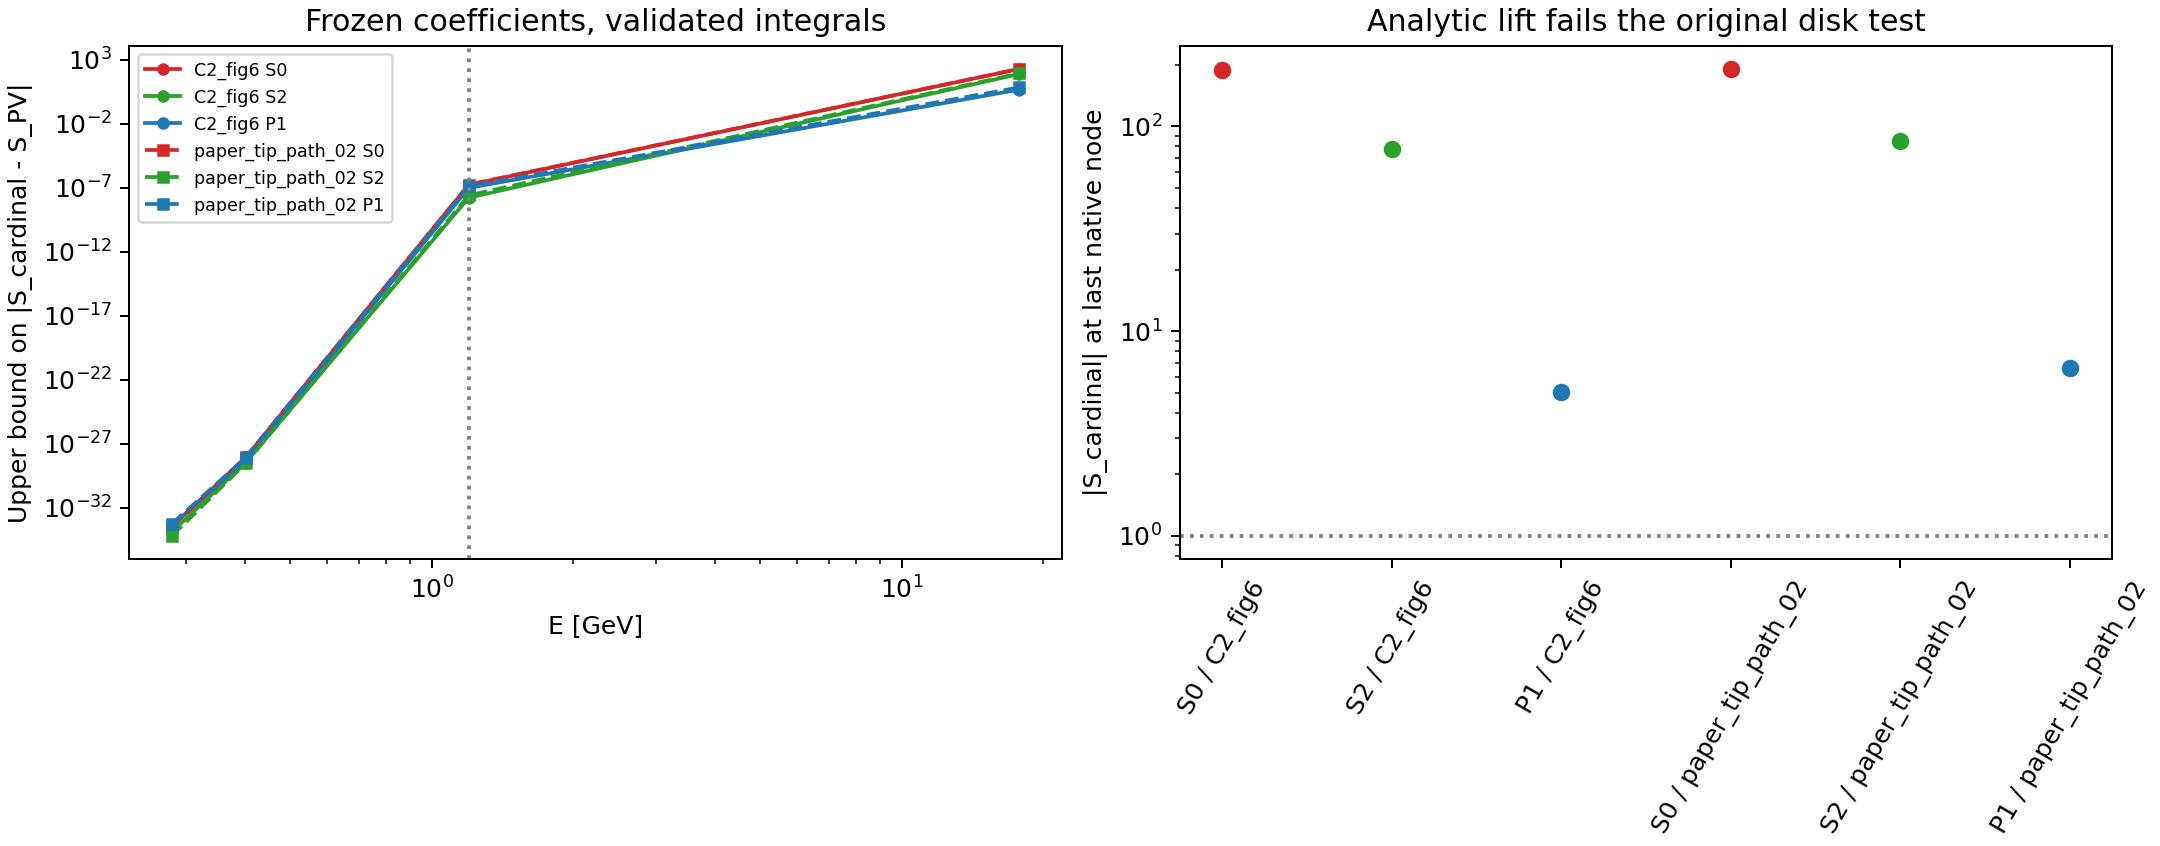
\includegraphics[keepaspectratio,alt={两种重建在相同冻结系数上的差异}]{verified_analytic_audit/analytic_comparison.png}}
\caption{两种重建在相同冻结系数上的差异}
\end{figure}

图中的连线只连接四个预定检查点。它不是 PV 离节点相移曲线。

进一步从完整系数和核差推得\textbf{整个4\textless s≤s₀范围}的保守误差界：

{\def\LTcaptype{none} % do not increment counter
\begin{longtable}[]{@{}lrrr@{}}
\toprule\noalign{}
向量 & S0 的 \(\lvert\delta S\rvert\) 上界 & S2 上界 & P1 上界 \\
\midrule\noalign{}
\endhead
\bottomrule\noalign{}
\endlastfoot
C2 & 2.539×10⁻⁵ & 1.088×10⁻⁵ & 7.601×10⁻⁶ \\
tip & 3.130×10⁻⁵ & 1.129×10⁻⁵ & 9.050×10⁻⁶ \\
\end{longtable}
}

这说明旧低能曲线的特征不只是绘图连线制造的，但\textbf{不能把低能求值接近推成优化可行域接近}：高能约束恰好参与了振幅的选择，而解析完成在这些节点被排除。

最高节点随M增长如 \(s_{\max}\sim64M^2/\pi^2\)。在那里
\(|z(4-s_{\max})|^M\to e^{-\pi/2}\)，Nyquist
混叠差不随M统一消失。离散L4界没有提供排除这类高频行为的假设。有限M/L图看似稳定不能替代这一缺失的误差论证。

数据与严格积分来源：\href{analytic_comparison/analytic_audit.json}{原始比较}、\href{verified_analytic_audit/analytic_audit.json}{统一界及留数}。

\subsection{3.
输入层的对齐与未解问题}\label{ux8f93ux5165ux5c42ux7684ux5bf9ux9f50ux4e0eux672aux89e3ux95eeux9898}

散射同位旋、8π²归一化、κ、M/L计数、实际ρ₂非对角除2、电流相空间因子、Gram共轭、FESR的π权以及平方FF界，都有独立推导与实现检查。L=10确实是每个同位旋十个波，不是最大角动量10。

但下列输入不能假称已经从理论唯一推出：

{\def\LTcaptype{none} % do not increment counter
\begin{longtable}[]{@{}
  >{\raggedright\arraybackslash}p{(\linewidth - 2\tabcolsep) * \real{0.5000}}
  >{\raggedright\arraybackslash}p{(\linewidth - 2\tabcolsep) * \real{0.5000}}@{}}
\toprule\noalign{}
\begin{minipage}[b]{\linewidth}\raggedright
项目
\end{minipage} & \begin{minipage}[b]{\linewidth}\raggedright
本轮审查
\end{minipage} \\
\midrule\noalign{}
\endhead
\bottomrule\noalign{}
\endlastfoot
χ 范数 &
2309写``某种范数''；combined-L2的历史选择确实使用了原Fig.5残差及后续代码，不能改写成自始独立的推导。两种L2集合的包含关系可证明，哪个是唯一原设置不能证明。 \\
E 选点 &
历史ref/mid使用了Fig.8输出标记坐标。固定在相位之前只避免相位择优，仍是参考输出参与设置。新选择接口已禁止该路径。 \\
夸克质量 &
共同平均质量代入Eq2.50，两个标量矩比打印目标低约8.48\%。RMS约低.68\%，但需改变/解释标量电流；不能因为数字更接近就采用。 \\
GMOR & 给定中心值的
\(-\langle j_S\rangle/(m_\pi^2f_\pi^2)=.6027931\)。凝聚中心值对应71.43MeV，而非92MeV。它们可以作为不同近似输入使用，不能声称精确LO自洽。 \\
SR误差 & raw
.002是声明的数值窗口，未由被遗漏OPE项或duality误差严格推出。标量一阶矩约8.5\%的中心差并不被原.002窗口覆盖。 \\
FF渐近 & 有限高能cap不是 \(F\to0\)
的证明。tip的最小次数FF完成在无穷远约为 .06813/.01858。 \\
正则化 &
B=100Nρ足以控制当前有限散射坐标，不是QCD唯一规定，也未证明对相位无影响。 \\
\end{longtable}
}

以上差异全部保留。没有修改凝聚、质量、s₀、范数或FF阈值来让曲线更像论文。

\subsection{4. A1--F3 全部核心 claim
的判定}\label{a1f3-ux5168ux90e8ux6838ux5fc3-claim-ux7684ux5224ux5b9a}

``有限已证''只针对明确给定的矩阵问题；``观察''不等于对全可行集的定理。

{\def\LTcaptype{none} % do not increment counter
\begin{longtable}[]{@{}
  >{\raggedright\arraybackslash}p{(\linewidth - 4\tabcolsep) * \real{0.3333}}
  >{\raggedright\arraybackslash}p{(\linewidth - 4\tabcolsep) * \real{0.3333}}
  >{\raggedright\arraybackslash}p{(\linewidth - 4\tabcolsep) * \real{0.3333}}@{}}
\toprule\noalign{}
\begin{minipage}[b]{\linewidth}\raggedright
步骤
\end{minipage} & \begin{minipage}[b]{\linewidth}\raggedright
成立的论证/证据
\end{minipage} & \begin{minipage}[b]{\linewidth}\raggedright
不能升级的结论
\end{minipage} \\
\midrule\noalign{}
\endhead
\bottomrule\noalign{}
\endlastfoot
A1 & 交叉/同位旋代数、完整参数计数已证；混合核的精确关系及留数障碍已证 &
当前完整离切线函数与原生值是同一个精确解析振幅 \\
A2 & 树级手征投影、电流归一化、FESR变换及单位已推导 &
唯一χ/B/mq/SR处方；全部输入严格QCD自洽 \\
A3 & 24项独立严格PV角积分；一致解析完成及统一低能核差界 &
全能量/全自旋幺正；所有离散误差已经消除 \\
B1 & 原式弱对偶、自由列消元、L4支持与有限紧性已证，verifier新增前提检查
& 任意H都能套用同一消元式；对无限物理模型的严格界 \\
B2 & 既有38份有限支持与.00967577几何预算 & 原图/原作者可行集完全同一 \\
B3 & 同范数ε嵌套定理、部分包含/排除和严格右端缩小 &
六个区域全部达到.01；ε=.001公式点已判定 \\
C1 & 81点线性改善观察；本轮严格证明橙/绿变号区间内有零点 &
蓝色全区间无零点；采样误差等于连续误差 \\
C2 & C1→C2→C3完整向量身份保留 & 未指定一致重建时的完整解析振幅身份 \\
C3 & 冻结IR点的P1不足、S0/S2低能形态有数据 &
所有IR可行振幅都不含ρ；由四点χ严格推出全部相移 \\
D1 & 复Gram与实锥等价；Schur条件及退化面充要条件已证 &
Gram是完整QCD的充分条件；PSD必定弹性 \\
D2 & 四个有限矩、FF平方界实现；独立输入审计完成 &
两矩必定产生峰；数值误差窗是严格OPE误差条 \\
D3 & 4076维完整联合有限见证仍有效 &
受限初始化已优化全空间；已构造全局QCD解 \\
E1 & UV包含IR及严格缩小的有限证据 &
原图约5.35的强非对称已经复现；当前比值只在约{[}.9554,1.1804{]} \\
E2 & 旧三点有限支持完成；新接口使用源图无关几何规则 &
旧参考标记选点是独立预测；全部振幅唯一 \\
E3 & 三点ρ式峰、Gram预算、固定C的UV排除证书 &
唯一极点/宽度；三点定量稳健性全部符合论文 \\
F1 & 四组已验；新增L条件必须重验 &
缺L12时五组完成；τ\textgreater0就是不可行证明 \\
F2 & 四组分辨率差异有数据 & 有限组曲线稳定就是连续收敛定理 \\
F3 & 本轮补足证明、反例、源码和逐claim台账 &
全部Fig.3--11及物理claim已完成 \\
\end{longtable}
}

本轮严格零点符号为：橙色 f₀⁰(.3)\textless0、f₀⁰(.35)\textgreater0；绿色
f₀⁰(.4)\textless0、f₀⁰(.45)\textgreater0。由离切线函数在对应区间连续，介值定理保证零点存在。没有把这个存在性论证冒充唯一性或蓝色无零点证明。

固定C的UV排除界仍约−9.09881296；原tip原式支持仍达标。这两项重验说明旧有限证据没有被本轮架构反例整体抹掉。

\subsection{5.
已落实的实现修正}\label{ux5df2ux843dux5b9eux7684ux5b9eux73b0ux4feeux6b63}

\begin{enumerate}
\def\labelenumi{\arabic{enumi}.}
\tightlist
\item
  新增
  \texttt{analytic.py}：从离散正弦正交性、Cauchy积分和圆参数化重新构造数学对象，作严格比较。未恢复退休源码，未把旧sine证书转移到PV。
\item
  \texttt{select-gauge}
  拒绝用论文输出标记作为科学选点输入。旧选择和数据原样保留，历史输出辅助性质明确标注。
\item
  优化/区域操作必须显式声明 χ
  范数，取消隐含的答案辅助默认值。原combined结果仍只代表该声明集合。
\item
  原式证书现在先检查其自由列消元恒等式。新增反例是一个真正无界的自由目标，不能再被误报为有限界。
\item
  \texttt{evaluate}
  保存完整f的精确球编码，浮点裕量端点向外舍入。S=0或非有限时不伪造相位；F=0节点继续参与谱和矩预算，只从需要F/F*的诊断中分开处理。
\end{enumerate}

现为13个按科学职责组织的模块、仍为三个测试文件。没有为增加数量而添加同类测试；本轮新增四项独立检查，最终结果见
\url{verification.json}。

\subsection{6.
下一步必须回答的物理决策}\label{ux4e0bux4e00ux6b65ux5fc5ux987bux56deux7b54ux7684ux7269ux7406ux51b3ux7b56}

首先明确要复现的是声明的有限近似，还是一个具有完整解析函数的有限参数族。若要后者，必须统一直接道与交叉道的核，再求新的完整联合见证；原PV可行性不能继承。解析尾部、T₀与FF无穷远条件应由所选函数族推出后才施加，不能向PV随意搬运，也不能只把旧T₀改成零就宣称修好------P1本来不含常数T₀，其高能反例仍在。

新输入协议必须先说明：采用打印矩还是Eq2.50、标量电流与质量规则、GMOR作为关系还是带误差输入、χ范数和B、端点求积及理论误差范围。图形输出不能参与选择。可行性成立后再按独立几何目标求支持，固定完整向量后才看相位，最后完成原五组M/L比较。

本轮没有以一个小模型替代论文结果，也没有把``再加采样/再跑迭代''写成充分修复。当前已证结构障碍、未公开处方和未完成的数值任务必须分别处理。

\subsection{来源与重放}\label{ux6765ux6e90ux4e0eux91cdux653e}

\begin{itemize}
\tightlist
\item
  原文：\href{https://arxiv.org/html/2309.12402v3}{2309.12402v3}，本地43页PDF与TeX；本轮参考的是公式与假设，不把原图数值当新输入。
\item
  上轮专家报告与\href{../expert_response_20260910/RHO_MECHANISM_AUDIT_ZH.md}{上一轮机制审计}均保留；其有限证书范围继续有效。
\item
  \href{AUDIT_PLAN.json}{预声明}、\href{verified_analytic_audit/analytic_audit.json}{完整严格比较及输入审计}、\href{C1_orange_root/evaluation.json}{橙色零点}、\href{C1_green_root/evaluation.json}{绿色零点}。
\item
  \href{finite_tip_recheck/report.json}{有限tip重验}、\href{finite_C_exclusion_recheck/report.json}{固定C排除重验}。
\item
  统一入口：\texttt{python\ -m\ smatrix\_bootstrap.run\ analytic-audit}。使用
  \texttt{-\/-comparison-manifest}
  时复用已经验证的角积分，只补代数误差界/输入审计；全部参数与producer在各运行报告中。
\end{itemize}

\newpage

\section{2309v3
复现的基础推导、反例与证明边界}\label{v3-ux590dux73b0ux7684ux57faux7840ux63a8ux5bfcux53cdux4f8bux4e0eux8bc1ux660eux8fb9ux754c}

本文件逐项给出本轮使用的数学论证。结论中的``有限模型''指保存的矩阵、明确的范数/容差和列定节点；``连续理论''另需完整函数族、全部能量/自旋条件和理论输入误差。两者不混用。目标源为本地
\href{../../../references/2309.12402v3.pdf}{2309.12402v3}，主要对应
(2.7)--(2.12)、(2.33)--(2.56)、(3.58)--(3.75)。原文的数值观察不自动成为普遍定理。

\subsection{P1.
从手征拉氏量到散射归一化}\label{p1.-ux4eceux624bux5f81ux62c9ux6c0fux91cfux5230ux6563ux5c04ux5f52ux4e00ux5316}

以 \(U=\exp(i\tau_a\pi_a/f_\pi)\)
展开最低阶手征拉氏量，二次项给出规范归一化的 pion 场，四次项为

\[
\mathcal L^{4\pi}_2=\frac{(\pi\cdot\partial\pi)^2-\pi^2(\partial\pi)^2}{6f_\pi^2}
+\frac{m_\pi^2(\pi^2)^2}{24f_\pi^2}.
\]

取在壳四点顶点、使用动量守恒及 \(p_i^2=m_\pi^2\)，得到

\[
\mathcal M_{ab,cd}=\frac{s-m_\pi^2}{f_\pi^2}\delta_{ab}\delta_{cd}
+\frac{t-m_\pi^2}{f_\pi^2}\delta_{ac}\delta_{bd}
+\frac{u-m_\pi^2}{f_\pi^2}\delta_{ad}\delta_{bc}.
\]

论文采用 \(T=\mathcal M/(8\pi^2)\)。三个 SU(2) 不可约投影给出

\[
\begin{aligned}
T^0&=3A(s,t,u)+A(t,s,u)+A(u,t,s),\\
T^1&=A(t,s,u)-A(u,t,s),\\
T^2&=A(t,s,u)+A(u,t,s).
\end{aligned}
\]

\(t\leftrightarrow u\) 对应 \(\mu\mapsto-\mu\)，所以 I=0,2 只留偶波，I=1
只留奇波。由 Legendre 正交性，

\[
f^I_\ell=\tfrac14\int_{-1}^{1}P_\ell T^I\,d\mu,
\qquad T^I=2\sum_\ell(2\ell+1)f^I_\ell P_\ell.
\]

与标准 \(\mathcal M^I=32\pi\sum(2\ell+1)t^I_\ell P_\ell\) 比较得到
\(t_\ell=\pi f_\ell/2\)。因此

\[
S=1+2i\beta t=1+i\pi\beta f,\qquad\beta=\sqrt{1-4/s}.
\]

将树级 A 投影，依次使用 \(\int1\,d\mu=2\)、\(\int\mu^2d\mu=2/3\)，有

\[
f^0_0=\frac{2s-1}{16\pi^2F_\pi^2},\quad
f^2_0=\frac{2-s}{16\pi^2F_\pi^2},\quad
f^1_1=\frac{s-4}{48\pi^2F_\pi^2},\quad F_\pi=f_\pi/m_\pi.
\]

树级给出 S0/S2 阈值相移的正/负号和 P1 的 \((s-4)^{3/2}\)
小量行为。代码实际约束的是四个阈下点的两种线性残差，并非精确树级振幅。因此这些阈值性质不能不加误差分析地推广到每个可行振幅；x
与物理 \(f_\pi\) 的精确关系也不能仅凭比例约束推出。

\subsection{P2.
幺正盘、完整幺正性与局部充分性}\label{p2.-ux5e7aux6b63ux76d8ux5b8cux6574ux5e7aux6b63ux6027ux4e0eux5c40ux90e8ux5145ux5206ux6027}

对完整幺正算子作两 pion 投影 P，

\[
(PS_{\rm full}P)^\dagger(PS_{\rm full}P)
=P-PS_{\rm full}^\dagger(1-P)S_{\rm full}P\preceq P.
\]

单个弹性分波因此满足

\[
|S|\le1\iff\Delta=\kappa(2\operatorname{Im}f-\kappa|f|^2)\ge0,
\qquad\kappa=\pi\beta.
\]

仅要求 Im f≥0 不够。反过来，每个标量收缩 S 都可在该能量用

\[
\begin{pmatrix}S&\sqrt{1-|S|^2}\\\sqrt{1-|S|^2}&-S^*\end{pmatrix}
\]

作幺正扩张。这只证明局部概率解释可行，不构造跨能量解析、交叉一致、满足所有多粒子约束的
QCD 算子。η=1
是无其它出射通道概率的情形，不是原文施加的普遍硬约束。s=4、有限 f 时
S=1；阈下点不用物理幺正盘。

\subsection{P3. 电流归一化与 Gram
的精确内容}\label{p3.-ux7535ux6d41ux5f52ux4e00ux5316ux4e0e-gram-ux7684ux7cbeux786eux5185ux5bb9}

两体 Lorentz 不变相空间满足 \(\int d\Phi_2=\beta/(8\pi)\)。实 pion
基底中，标量矩阵元正比 \(\delta_{ab}F_0\)，同位旋求和与相同粒子因子给
\(3/2!\)。矢量矩阵元正比 \(\epsilon^{Iab}(p_2-p_1)_iF_1\)，求和后
\(2/2!=1\)，单个空间极化的角平均为
\(4|\mathbf p|^2/3=(s-4)/3\)。计入论文电流 Fourier 定义的
\((2\pi)^{-4}\)，得到

\[
\rho^{2\pi}_0=\frac{3\beta}{256\pi^5}|F_0|^2=k_0^2|F_0|^2,
\quad\rho^{2\pi}_1=\frac{(s-4)\beta}{384\pi^5}|F_1|^2=k_1^2|F_1|^2.
\]

这独立说明了三个易错因子：相同粒子的 1/2、标量同位旋的 3、单极化矢量的
1/3。矢量电荷给 F₁(0)=1；Feynman--Hellmann 与最低阶质量关系给
\(F_0(0)=m_q\partial m_\pi^2/\partial m_q\simeq m_\pi^2\)，在当前单位中取
1。这里的 F₀(0)≈mπ² 是最低阶近似；Feynman--Hellmann
的导数关系自身不因此失效。

令 \(a=\mathcal F=kF,\ R=\rho_{\rm current}\)。由三个态的 Gram 矩阵

\[
G=\begin{pmatrix}1&S&a\\S^*&1&a^*\\a^*&a&R\end{pmatrix}\succeq0
\]

作固定酉变换，可得代码使用的实矩阵

\[
G_R=\begin{pmatrix}1+\operatorname{Re}S&\operatorname{Im}S&\sqrt2\operatorname{Re}a\\
\operatorname{Im}S&1-\operatorname{Re}S&\sqrt2\operatorname{Im}a\\
\sqrt2\operatorname{Re}a&\sqrt2\operatorname{Im}a&R\end{pmatrix}.
\]

正对角数值均衡只是可逆合同变换。PSD 与三个向量的存在等价；这仍不是完整
QCD 的充分条件。

当 Δ\textgreater0 时直接求上方 2×2 块的 Schur 补：

\[
G\succeq0\iff
R\ge R_{\min}=|a|^2+\frac{|a-Sa^*|^2}{\Delta},\qquad
\det G=\Delta(R-|a|^2)-|a-Sa^*|^2.
\]

当 Δ=0 时，充要条件改为 \(a=Sa^*\) 且 \(R\ge|a|^2\)；a=0 时只剩 R≥0
和散射盘。故不能把有限精度下很小的 Δ 当作可安全相除的数。

若 F≠0，\(Q=F/F^*,r=|a|^2/R,S=\eta e^{2i\delta}\)，则

\[
|S-Q|^2\le(1-\eta^2)(r^{-1}-1),
\quad4\eta\sin^2(\delta-\arg F)
\le(1-\eta^2)(r^{-1}-1)-(1-\eta)^2.
\]

两 pion 谱完全饱和强制弹性 Watson 关系；弹性本身不强制谱完全饱和。det
G≈0 可以只是 Schur 下界接近饱和。对任意正 FESR 权，谱矩精确分成``两 pion
+ 必须支付的失配代价 + 非负剩余''。这是 UV 传递到同一 S 的确切数学通道。

\subsection{P4. 高能输入与
FESR：精确变换和近似输入分开}\label{p4.-ux9ad8ux80fdux8f93ux5165ux4e0e-fesrux7cbeux786eux53d8ux6362ux548cux8fd1ux4f3cux8f93ux5165ux5206ux5f00}

自由夸克切割可核对领先项：标量自旋和为
\(2s\)，单个矢量空间极化的角平均为 \(4s/3\)。乘相空间、颜色及味道权重，

\[
\rho_S\sim\frac{N_c\sum_f c_f^2}{(2\pi)^4}\frac{s}{4\pi},\qquad
\rho_V\sim\frac{N_c\sum_f q_f^2}{(2\pi)^4}\frac{s}{6\pi}.
\]

论文取共同 \(c_f=m_q\) 和
\(q_u=-q_d=1/2\)，恰好还原论文领先阶夸克圈的对数系数。改变为 \(c_f=m_f\)
才产生 \(\sum m_f^2\)；这改变了标量电流，不能因 RMS
更接近打印数字就宣称它一定是同一个 I=0 电流。

以 \(\rho=2\operatorname{Im}\Pi\)，Cauchy 定理给

\[
M_n=\int_4^{s_0}\rho(x)x^n dx
=i\oint_{|s|=s_0}s^n\Pi(s)ds
=-s_0^{n+1}\int_0^{2\pi}e^{i(n+1)\phi}\Pi(s_0e^{i\phi})d\phi.
\]

在割线约定 \(\log(-s/\mu^2)=\log(s_0/\mu^2)+i(\phi-\pi)\) 下，

\[
\Pi=-c\,s\log(-s/\mu^2)+d/s
\quad\Longrightarrow\quad
M_n=\frac{2\pi c\,s_0^{n+2}}{n+2}-2\pi d\,\delta_{n0}.
\]

因此代入论文 (2.47) 的 Wilson 系数即得 (2.50)，无需参考相移或峰位。n=−1
的矢量矩另需 Π₁(0)=0，不能忽略原点残项。NLO 的 13/3
等系数在此作为具名高能理论输入；本轮没有声称独立重算全部两回路图和 OPE
余项。

精确 FESR 对真实 Π 成立。若圆上误差为 δΠ，则

\[
|\delta M_n|\le2\pi s_0^{n+1}\sup_{|s|=s_0}|\delta\Pi(s)|.
\]

当前 .002 是有限约束的声明容差，没有上述 QCD
余项上界，不能称为严格物理误差条。标量 NLO 相对领先项约 55\%，矢量约
13\%；对更高阶误差不能凭``微扰''二字设为零。

物理标量/矢量谱分别除以 \(m_\pi^4,m_\pi^2\)，四个 raw 矩依次除以
\(m_\pi^{6,8,2,4}\)。F₀ 除以 \(m_\pi^2\)，F₁ 不变。FESR 权含
\((\pi/M)x'_i\)，散射 Cauchy 核则已含 1/π，权为 \(x'_i/M\)。FF 界施加于
\(k^2|F|^2\)，不能改成同数值的 \textbar F\textbar{} 或
\textbar F\textbar² 界。

输入审计实测：GMOR 中心值比
\(-\langle j_S\rangle/(m_\pi^2f_\pi^2)=0.6027931\)，由给定凝聚得到的 fπ
为 71.43 MeV，并非 92 MeV。按共同平均质量计算的两个标量矩比打印目标低约
8.48\%；RMS 差约
.68\%，但不构成电流同一性的证明。这些是近似输入的真实差异，不在本轮偷偷修正。

\subsection{P5. 不能从矩、模长或 90°
上穿推出唯一谱}\label{p5.-ux4e0dux80fdux4eceux77e9ux6a21ux957fux6216-90-ux4e0aux7a7fux63a8ux51faux552fux4e00ux8c31}

\(M_0/M_{-1}\) 是正测度 \(R(s)ds/s\) 下的 s
平均值，只有另加窄峰饱和假设才近似为质量平方。当前 M50 的两个 P1
离散中心值可由

\[
R_i=a+b s_i,\quad
a\simeq7.25782151648\times10^{-4},\quad
b\simeq2.53523484779\times10^{-5}
\]

精确满足；Arb 解出的 a,b
严格为正，所以它单调上升且无内峰。此反例针对``两矩本身足够''的命题，没有冒充全部联合约束的反例。

即使知道完整模长、F(0) 和领先衰减，解析性也不总唯一确定相位。取

\[
P(z)=1-z+\tfrac{17}4z^2-4z^3+z^4,\quad
P^\#(z)=z^4P(1/z),
\] \[
F(z)=(1+z)^2P(z),\qquad\widetilde F(z)=(1+z)^2P^\#(z).
\]

两者实系数、F(0)=1、在 z=−1 有双零点，领先 \(1/s\) 系数相同；单位圆上
\(|P^\#|=|P|\)，但一般相位不同。共同的解析因子不会消除这个歧义。零点/内因子信息不能省略；该反例也没有声称两者已满足完整
pion 交叉约束。

散射强度为 \(I=|S-1|^2/4=(1+\eta^2-2\eta\cos2\delta)/4\)。δ=π/2 处
\(I'=(1+\eta)\eta'/2\)，所以非弹性变化会使强度峰偏离 90°。S=0
时相位无定义。有限节点的 unwrap 还需分支约定；它不是第二张面极点证明。

\subsection{P6. 有限 Hilbert
核与有理求积核的精确关系}\label{p6.-ux6709ux9650-hilbert-ux6838ux4e0eux6709ux7406ux6c42ux79efux6838ux7684ux7cbeux786eux5173ux7cfb}

设

\[
\begin{gathered}
\phi_j=\pi(j+1/2)/M,\quad x_j=4/\cos^2(\phi_j/2),\quad w_j=x'_j/M,\\
z(s)=\frac{2-\sqrt{4-s}}{2+\sqrt{4-s}},\qquad s=\frac{16z}{(1+z)^2}.
\end{gathered}
\]

当前离切线核严格等于

\[
q^R_j(s)=\frac{w_js}{x_j(x_j-s)}
=\frac{2z\sin\phi_j}{M(1-2z\cos\phi_j+z^2)}
=\frac2M\sum_{n\ge1}z^n\sin(n\phi_j).
\]

由离散正弦正交性，给定节点密度 v，唯一的 M
次以内实系数、零常数解析多项式为

\[
P_M(z)=\sum_{n=1}^M a_nz^n,\qquad
a_n=\frac{2-\delta_{nM}}M\sum_jv_j\sin(n\phi_j).
\]

它在原生节点满足 Im P=v、Re P=Kv，K 正是论文 (3.67)；Nyquist 模 n=M
必须保留，且权重为其余模的一半。直接对连续 Cauchy
积分作正弦正交展开也得到 \(z^n\)。

但离切线求积包含所有混叠模。利用

\[
\sin((2M-n)\phi_j)=\sin(n\phi_j),\quad
\sin((2M+n)\phi_j)=-\sin(n\phi_j),
\]

求和得到精确公式

\[
R_M(z)=\sum_jq^R_jv_j
=\frac{\sum_{n=1}^{M-1}a_n(z^n+z^{2M-n})+2a_Mz^M}{1+z^{2M}}.
\tag{A}
\]

因此当前边界使用 P\_M，离切线使用 R\_M；两者一般不等。M50 的单核差在 s=3
约≤5.57×10⁻²⁶，在 s=−100
已约为2.38×10⁻¹⁰。不能因阈下很小就认定整个物理约束网格误差也小。

无减法坐标也没有被偷换：由有限三角和可证
\(P_{M,j}(-1)=-w_j/x_j\)，故两种无减法核共享同一个
b\_j=w\_j/x\_j。代码的完整 σ、ρ 与 T₀
减法换元可精确用于这个比较，未删除任何变量。

\subsection{P7.
共同解析振幅的障碍：极点留数证明}\label{p7.-ux5171ux540cux89e3ux6790ux632fux5e45ux7684ux969cux788dux6781ux70b9ux7559ux6570ux8bc1ux660e}

在任一原生正实点 xᵢ 附近，离切线公式的部分波可写成

\[
f_R(s)=B(s)+\sum_j\frac{w_j}{x_j-s}A_j(s),
\]

其中交叉道参数 t,u≤0，使 Aⱼ、B 在 xᵢ
邻域解析且在实轴为实数。当前原生规则把第 i 个直接核的虚部指定为 1，因此

\[
\boxed{\operatorname{Res}_{s=x_i}f_R(s)=-w_i\operatorname{Im}f_{PV}(x_i).}
\tag{B}
\]

只要该虚部非零，离切线函数的解析延拓便有非零极点，不可能同时取得程序指定的有限节点值。若另一个解析函数与已定义的整个阈下函数相同，恒等定理迫使其延拓也相同；不能另行指定有限边界值来消去极点。本轮两个冻结振幅的24个检查点全部具有经区间确认的非零留数。

在非节点正实能量上，这个有理延拓的部分波为实数；只要它不为零，就有
\textbar1+iκf\_R\textbar²\textgreater1。因此问题不只是极点处的一种显示约定。

这个结论针对``现有完整离切线求值与原生值属于同一个精确解析函数''的命题。若只保留有限个采样数、允许更换插值族，则其它解析完成是否存在是另一问题。它不证明所有可能的解析完成都不存在，也不证明论文未公开程序必然与当前相同。

\subsection{P8.
局部误差、移动网格与严格角积分}\label{p8.-ux5c40ux90e8ux8befux5deeux79fbux52a8ux7f51ux683cux4e0eux4e25ux683cux89d2ux79efux5206}

对 \textbar z\textbar≤r\textless1，(A) 减 P\_M 后，各模可保守界定为

\[
e_n=\frac{r^{2M-n}+r^{2M+n}}{1-r^{2M}}\ (n<M),\qquad
e_M=\frac{r^M(1+r^{2M})}{1-r^{2M}}.
\]

固定紧集上有指数抑制；但最高节点

\[
x_{M-1}\sim64M^2/\pi^2,\quad
r_M=|z(4-x_{M-1})|=\frac{1-\sin(\pi/(4M))}{1+\sin(\pi/(4M))},
\quad r_M^M\to e^{-\pi/2}.
\]

单位 Nyquist 模在该移动网格端的差趋于
\(e^{-\pi/2}\tanh(\pi/2)>0\)。这证明在允许高频密度的函数族上没有所需的统一核误差消失；不等于声称每个固定光滑密度都不收敛。离散
L4 界不提供统一导数/高频衰减假设。

对固定完整系数，转到模坐标后同位旋振幅为
\(c+L(p_t\pm p_u)+p_t^T K_Ip_u\)。令 \(u_n=r^n\)，用上述 e、L
的绝对值上界和 \(|P_\ell(\mu)|\le1\)，得到

\[
|\delta f_\ell^I|\le\sum_j\overline L_j e_j+
\frac12\sum_{ij}|K_{I,ij}|(u_i e_j+e_i u_j+e_i e_j).
\tag{C}
\]

对4\textless s≤s₀，取
\(r=(\sqrt{s_0}-2)/(\sqrt{s_0}+2)=23/37\)，便是本轮
uniform\_error\_bound 的完整证明。乘π即得 S
的上界。该比较在两侧均使用同一直接边界多项式，不冒称定义了唯一的 PV
离节点延拓。

角积分的独立核验没有使用生产 Legendre-Q 投影。置 R=√(s+4)，

\[
x=R\frac{1-q^2}{1+q^2},\quad y=R\frac{2q}{1+q^2},\quad
t=4-x^2,\quad u=4-y^2,
\] \[
q_-={2\over R+\sqrt s},\quad q_+={\sqrt s\over R+2},\quad
{1\over4}{d\mu\over dq}={4(s+4)q(1-q^2)\over(s-4)(1+q^2)^3}.
\]

此时
z(t)=(2−x)/(2+x)、z(u)=(2−y)/(2+y)，所有被积函数都是q的有理函数。Arb
的复积分能验证解析邻域并包住积分余项；没有忽略移动平方根的分支。M50
两个振幅、四个预定节点、三个主波，PV
的24项独立积分均与闭式投影相交；另一种重建的24项积分也得到有限窄包络。

\subsection{P9.
一致解析完成的尾部结论和它的适用范围}\label{p9.-ux4e00ux81f4ux89e3ux6790ux5b8cux6210ux7684ux5c3eux90e8ux7ed3ux8bbaux548cux5b83ux7684ux9002ux7528ux8303ux56f4}

最小次数的正弦/多项式完成在无减法坐标下满足单核
H(∞)=0，且有限多项式在闭单位盘有界。固定角度令s→∞，除零测度端点外 s,t,u
都趋向无穷；支配收敛给

\[
f^0_0(\infty)=\tfrac52T_0,\quad f^2_0(\infty)=T_0,\qquad
\Delta^0_0(\infty)=-\pi^2(5T_0/2)^2.
\]

所以该完成若要全能量幺正，T₀=0
是必要条件，仍非充分条件。不能把它直接加到未指定相同尾部的 PV
模型。原文一般密度/Regge
尾部若不满足这个有界性假设，也不能借此交换极限与角积分。

该最小次数 FF 的极限为 \(F(-1)=1-\sum_jb_j\operatorname{Im}F_j\)。tip
得到标量 .0681255、矢量 .0185755，并非零。F(∞)=0
和至少1/s衰减分别需要这个完成的 F(−1)=0、F′(−1)=0；七个有限高能 cap
不推出这些等式。

更高次数的解析补项可以在全部原生节点和z=0处消失、同时修正z=−1的条件。因此这些尾部反例针对声明的最小次数完成，不是所有
FF 完成的不可行证明。已有完整离切线散射函数的障碍则由 P7
的恒等定理另外处理。

\subsection{P10.
正则化、有限支持与数值中心}\label{p10.-ux6b63ux5219ux5316ux6709ux9650ux652fux6301ux4e0eux6570ux503cux4e2dux5fc3}

令 r 为实际双谱独立条目，非对角 C\_flat 先除2，且
\(\lVert r\rVert_4\le B<\infty\)。原生虚部恒等式为

\[
u_{0i}=\tfrac32\sigma_{1i}+\sigma_{2i}+D_{0i}r,\quad
u_{2i}=\sigma_{2i}+D_{2i}r,
\quad0\le u_{0i},u_{2i}\le2/\kappa_i.
\]

故 Hölder 给

\[
|\sigma_{2i}|\le2/\kappa_i+B\|D_{2i}\|_{4/3},\quad
|\sigma_{1i}|\le4/(3\kappa_i)+(2B/3)\|D_{0i}-D_{2i}\|_{4/3}.
\]

任取实 S0 行 \(\operatorname{Re}f=5T_0/2+a\sigma+Dr\)，由 \textbar Re
f\textbar≤1/κ
又界定T₀。固定M下全部系数有界，约束闭、零振幅可行，所以散射集紧、线性支持取得最大值。不要求整个H满列秩，不借用历史
sine 秩证明。B=100Nρ 是声明的离散配方，不能从 QCD
唯一推出，也不提供连续密度正则性。

散射盘的支持函数为 \(\sqrt{k_R^2+k_I^2}+k_I\)，手征球的支持函数为
ε‖y‖₂，密度球的支持函数为
B‖r\_dual‖₄/₃。把目标减去这些线性协变量，用上述原生恒等式消去自由 T₀、σ
残差，就得到原始坐标的合法上界。联合情形增加 PSD、FESR、FF
协变量及常数，剩余 current
残差用这些原约束推出的变量界控制。该弱对偶证明不依赖求解器的成功标签或
Slater 条件。

这一证明有代数前提。本轮 verifier 增加了对完整 H 形状、有限性、正 κ
和原生自由列恒等式的检查。若把 σ₁
从所有约束中删除、却仍用它作目标，问题显然无界；旧的固定消元式可能错误给出有限上界，新检查拒绝这种矩阵。

在严格内点，正权 log barrier 对密度变量、原生自由列、current/FF
变量的曲率共同消除非零零方向，因此中心问题严格凸。可逆坐标变换、正障碍权重不改可行集，但有限μ的选点和极限面选择仍需记录。收敛中心与任意可行混合不是同一个概念。支持
gap 控制线性目标；没有额外强暴露/观测量界时不控制整个振幅或相位。

\subsection{P11.
联合集的闭包、固定振幅证书与凸组合}\label{p11.-ux8054ux5408ux96c6ux7684ux95edux5305ux56faux5b9aux632fux5e45ux8bc1ux4e66ux4e0eux51f8ux7ec4ux5408}

低能R由正矩权上界控制，低能F由Gram主子式控制，高能F由cap控制。高能R仍可无界。若高能Δ\textgreater0，可按Schur下界补出有限R；Δ=0另需范围条件。故不能把散射紧性直接推广到完整联合变量。

例如S↗1、固定非零纯虚F时，所需R\_min发散，而端点不满足Watson范围条件。在存在高能盘严格内点的条件下，将其与任一消去高能R后的点作凸混合，再补R，证明紧松弛集合是原投影闭包、线性支持上确界相同；不保证每个边界上确界由有限R取得。

固定完整C后，合法对偶及残差支持给
\(0\le U_C\)。严格负的U\_C就排除该C的所有 current
扩展。本轮/上一轮约−9.09881296的证书是这一命题；既非完整问题不可行，也非所有无ρ振幅被排除。对偶射线可缩放，其数值不是物理距离。

两个完整联合可行点的凸组合仍可行，因为所有Γ、F与矩都是同一完整变量的仿射映射。把一个联合点整体径向缩放却没有此保证：F(0)=1不是齐次约束。散射-only
的原点混合则由盘凸性和齐次χ/密度界保证。

\subsection{P12.
区域、零点、分辨率及``全部核心claim''的量词}\label{p12.-ux533aux57dfux96f6ux70b9ux5206ux8fa8ux7387ux53caux5168ux90e8ux6838ux5fc3claimux7684ux91cfux8bcd}

同一模型中 ε
缩小给集合嵌套；加入UV给投影包含。严格缩小需一个旧可行值超过新支持上界，或截面内外界严格分离。可行点凸包是内包，所有合法支持半平面的交是外包。到凸集的距离是凸函数，所以对外多边形全部顶点的距离上界控制整个多边形；.01
几何预算与原图误差、相位误差是不同概念。

橙/绿 S0 的两个端点本轮以完整 Arb
包络确认异号；离切线核在相应阈下闭区间连续，因此介值定理给出至少一个零点。蓝色的有限采样没有变号不能证明整个区间无零点，有限采样上的线性改善也不能升级为统一函数误差界。

固定M增加L时，共享算子完全相同才有约束集合的嵌套。改变M同时改变变量、节点、求积和B，不能继承可行性。四个配置不能替代五个；有限个配置的曲线接近也不是M,L→∞的收敛证明。当前L12无见证、也无原式不可行证书；E的定量差异同样未消失。

因而可补全的是上面每个成立的条件命题及其数值证据。不能为已发现反例的``共同精确解析振幅''、或尚缺计算/理论误差的``全部论文结果、唯一QCD谱和连续认证''补造证明。

数值、代码修正、A1--F3台账与原始运行路径见
\href{REVIEW_ZH.md}{本轮审查}。新角积分来自重新推导的
\texttt{analytic.py}，没有恢复退休模块，也没有导入旧 sine
可行性或秩结论。

\end{document}
